\documentclass[a4paper,12pt,chapterprefix=false,bibliography=totoc,listof=totoc,]{scrreprt}

% Benannte Farben
\usepackage{xcolor}
% Schriftauswahl
\usepackage{fontspec}
% Spracheinstellungen
\usepackage[english]{babel}
% Grafiken einfügen
\usepackage{graphicx}
% [H] Platzierung
\usepackage{float}
% Tabellen
\usepackage{tabu}
% KOMA-Script Mods für float,hyperref,listings,setspace
\RequirePackage{scrhack}
% hyperref als letzes
\RequirePackage{hyperref}
\hypersetup{
    colorlinks=true,
    linkcolor=blue,
    filecolor=magenta,      
    urlcolor=cyan,
}
% Glossareinträge nach hyperref
\RequirePackage[toc, style=altlist, nonumberlist, abbreviations, xindy]{glossaries-extra}

% Füge andere Abkürzungen
\newabbreviation{k8s}{K8S}{Kubernetes}
\newabbreviation{aws}{AWS}{Amazon Web Services}
\newabbreviation{tbd}{TBD}{To be determined}
\newabbreviation{na}{N/A}{Not applicable}
\newabbreviation{dto}{DTO}{Data Transferable Object}
\newabbreviation{stc}{STC}{Subject to change}
\newabbreviation{gcs}{GCS}{Google Cloud Services}
\makeglossaries

\setlength{\parindent}{0pt}

\begin{document}	
\begin{flushright}
GameBase
\\
Software Requirements Specification
% \\
% For <Subsystem or Feature>
\bigbreak
Version 1.0
\end{flushright}
\chapter*{Revision History}
\begin{table}[H]
	\centering
	\everyrow{\hline}
	\begin{tabu} to \textwidth {|X[c]|X[c]|X[c]|X[c]|}
		Date & Version & Description & Author\\
		10/23/2019 & 0.1 & Added Use Case Diagram & Norman Gehrsitz \\
		10/28/2019 & 0.2 & Added Activity Diagram for creating and configuring game server & Leonhard Gahr \\
		10/xx/2019 & 1.0 & Complete current state of information & Kevin Reis \\
		<mm/dd/yyyy> & <x.x> & <details> & <name>\\
	\end{tabu}
	\label{tab:rev-hist}
\end{table}

\tableofcontents

\chapter{Introduction}
%[The introduction of the Software Requirements Specification (SRS) should provide an overview of the entire SRS. It should include the purpose, scope, definitions, acronyms, abbreviations, references, and overview of the SRS.]

% [Note: The Software Requirements Specification (SRS) captures the complete software requirements for the system, or a portion of the system.  Following is a typical SRS outline for a project using only traditional natural-language style requirements – with no use-case modeling.  It captures all requirements in a single document,  with  applicable sections inserted from the  Supplementary Specifications (which would no longer be needed).  For a template of an SRS using use-case modeling, which consists of a package containing Use-Cases of the use-case model and applicable Supplementary Specifications and other supporting information, see rup\_SRS-uc.dot.]

% [Many different arrangements of an SRS are possible.  Refer to [IEEE830-1998] for further elaboration of these explanations, as well as other options for SRS organization.]

\section{Purpose}
% [Specify the purpose of this SRS. The SRS should fully describe the external behavior of the application or subsystem identified. It also describes nonfunctional requirements, design constraints and other factors necessary to provide a complete and comprehensive description of the requirements for the software.]
The purpose of this document is to give a general description of the GameBase project. It explains our vision and all features we plan to provide. It is supposed to offer insights into the system in terms of back- and frontend, the interfaces in both ends for communication and the constraints of the system.

\section{Scope}
% [A brief description of the software application that the SRS applies to; the feature or other subsystem grouping; what Use-Case model(s) it is associated with;  and anything else that is affected or influenced by this document.]
\subsection*{Target group}
We want to offer our software to everyone who wants easy game server management and deployment without heavily modifying their system. It can be also used in an commercial environment like hosting game server services to other people.

\subsection*{Components}
This software is divided into two obvious components
\begin{itemize}
	\item Frontend (End-user server management)
	\item Backend (Deployment to specified destination, Docker Image creation)
\end{itemize}


\section{Definitions, Acronyms and Abbreviations}
\printabbreviations[title={}]

\section{References}
\begin{table}[H]
	\centering
	\everyrow{\hline}
	\begin{tabu} to \textwidth {|X[c]|X[c]|X[c]|}
		\textbf{Title} & \textbf{Date} & \textbf{Author} \\
		\href{https://gitlab.tandashi.de/GameBase}{Git Repository} & 10/23/2019 & GameBase \\
		\href{https://youtrack.gahr.dev}{YouTrack} & 10/23/2019 & GameBase \\
		\href{https://gahr.dev}{Blog} & 10/23/2019 & GameBase \\
		\href{https://www.docker.com/}{Docker} & 10/23/2019 & Docker Inc. \\		
	\end{tabu}
	\label{tab:references-tabview}
\end{table}

\section{Overview}
% [This subsection should describe what the rest of the SRS contains and explain how the document is organized.]
The next chapters provide information about our vision based on a use case diagram as well as more detailed software requirements. Additionally, we are going to outline the steps required to comply with legal requirements and technical standards.

\chapter{Overall Description}
\section{Vision}
% [This section of the SRS should describe the general factors that affect the product and its requirements.  This section does not state specific requirements.  Instead, it provides a background for those requirements, which are defined in detail in Section 3, and makes them easier to understand. Include such items as:
% \begin{itemize}
% 	\item product perspective
% 	\item product functions
% 	\item user characteristics
% 	\item constraints
% 	\item assumptions and dependencies
% 	\item requirements subsets
% \end{itemize}]
Setting up game servers can be painful. Either way when hosting on a dedicated server, you need to get into e. g. Bash where things could get messy really fast if you don't have enough experience. And in case you want to get rid of your installed unsteady server, you also need to take care of removing all remaining files that sit somewhere in your file system. Good luck on that!

With GameBase, we want to make your game server deployment life way easier. Using Docker – a state-of-the-art virtualisation technology – servers can be set up through templates on a website and ready to be deployed with just one click. This also makes sure that every game server is isolated from each other avoiding possible conflicts with each other as well.

\section{Product perspective}
\begin{figure}
	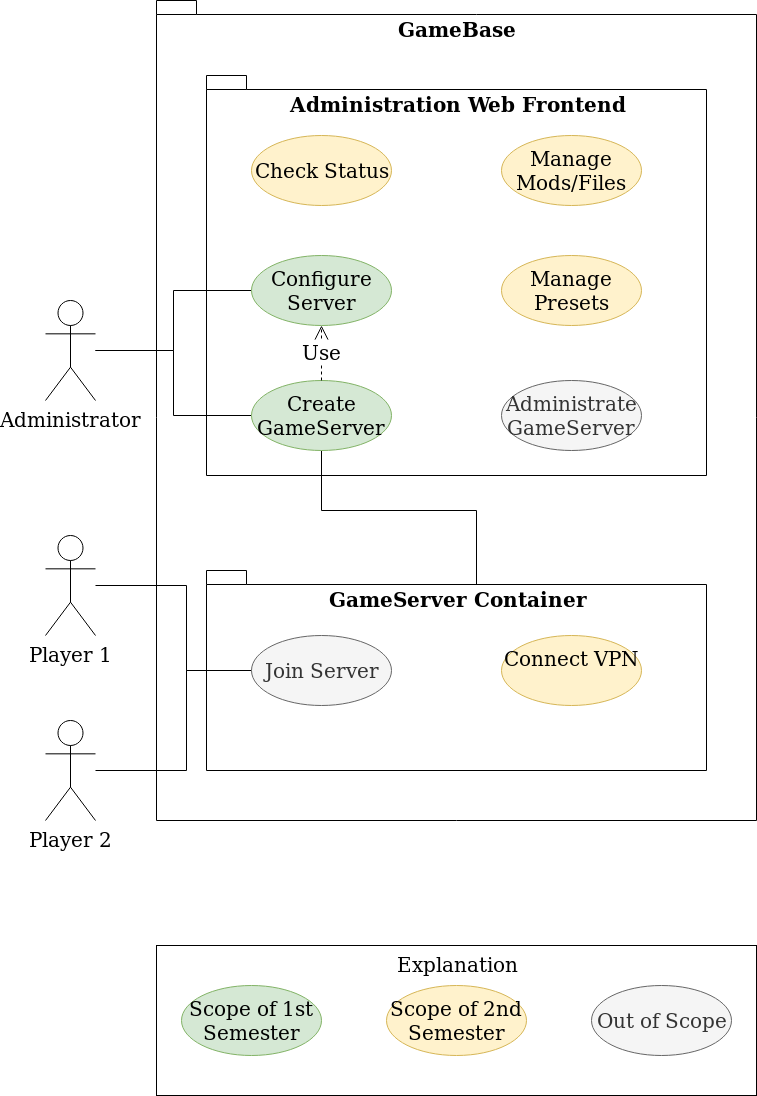
\includegraphics[width=\textwidth]{Use_Case_Diagramm.png}
	\caption{Use Case Diagramm}
	\label{fig:ucd}
\end{figure}
Players are featured in our diagram even though they are not interacting with our application directly because after all connecting to the servers is a crucial part of our system.

Administration of the game servers with game specific features like \emph{kicking}, \emph{banning} and \emph{map rotation} is out of scope. This is due to the variety of games and their systems that handle these actions independently. As we want to offer an experience of settings up any kind of game servers

The main use cases of our application are managing the game server containers.
As such creation and configuration of severs is the milestone for our first semester, whereas status reporting, managing server files, ((((((enabling network access to the containers network ))))))and managing server presets is in scope for the second semester.

\chapter{Specific Requirements}
% [This section of the SRS should contain all the software requirements to a level of detail sufficient to enable designers to design a system to satisfy those requirements, and testers to test that the system satisfies those requirements.   When using use-case modeling, these requirements are captured in the Use-Cases and the applicable supplementary specifications.  If use-case modeling is not used, the outline for supplementary specifications may be inserted directly into this section, as shown below.]

\section{Functionality - Backend}
% [This section describes the functional requirements of the system for those requirements which are expressed in the natural language style. For many applications, this may constitute the bulk of the SRS Package and thought should be given to the organization of this section. This section is typically organized by feature, but alternative organization methods may also be appropriate, for example, organization by user or organization by subsystem.  Functional requirements may include feature sets, capabilities, and security.

% Where application development tools, such as requirements tools, modeling tools, etc., are employed to capture the functionality, this section document will refer to the availability of that data, indicating the location and name of the tool that is used to capture the data.]

The backend's task is to orchestrate Docker container. The orchestration method depends on the selected deployment. It can either be native or a 3rd party provider like \gls{k8s} or \gls{aws}. The user can choose a Docker image on the frontend side, and the backend takes care of it being deployed as a container.

\subsection{Server management and creation (3rd semester)}
Through the frontend the user should be able to create any kind of game server containers and manage them. The image can either be:
\begin{itemize}
	\item an already built one 
	\item or be built by \emph{Dockerfile}.
\end{itemize}
 
 
The functionality of management contains:
\begin{itemize}
	\item Start, stop and kill server
	\item Create container
	\item Configuring server (ports, player slots, RAM usage, ...)
	\item Select deployment method
	\item Recreating container (equals reinstallation)
\end{itemize}

\subsection{Status reporting (4th semester)}
For better troubleshooting and further, concise information about a user's container, a status reporting system will be introduced. Example status can be:
\begin{itemize}
	\item Building...
	\item Starting...
	\item Running
	\item Stopping...
	\item Stopped
\end{itemize}

\subsection{Volume management (4th semester)}
The client should be able to access server files inside a container via FTP/SFTP. This functionality can also include backup server files and make restoring accessible through the frontend.

\subsection{User system (3rd + 4th semester)}
At registration, the data provided by the user is stored in the backend. It is needed to log in, edit the profile and also provides the basis for a permission system. According use cases are:

\begin{itemize}
	\item Register
	\item Log in
	\item Log out
	\item Change profile
	\item Delete profile
\end{itemize}

As of defined use case scopes, in the 3rd semester, we firstly stick to only one account with Basic authentication.

\subsection{Preset registry ((3rd +) 4th semester)}
Searching Docker images can be a hassle for Docker-inexperienced users. This is why it makes sense to provide a preset registry not only for pre-built, but also for user-created images and Dockerfiles. This reduces effort of creating multiple servers with images that have been built in the past.

The backend is needed to separate the user interface from the data storage. It verifies if the correct permissions are present to request data or to ensure that incoming data is properly parsed and saved correctly. For security reasons data is filtered by the backend. It is then packed in the right format which the next chapter describes. The data is kept inside a database and maintained by the backend.

% \subsection{<Functional Requirement One>}
% [The requirement description.]

\subsection{Read and parse data passed by API endpoints}
For the communication between both sides (frontend and backend) a universal data format is needed, therefore JSON is used. The frontend sends data in JSON to the backend in form of a request via an HTTP client and waits for a response from the backend which also answers with JSON.

It's important to validate input and output data in order to avoid malfunctions or possible abuse of undetected bugs. In case of sharing \gls{dto} files we need to make sure that we have a centralized module which can be added as dependency by any component.

\subsection{Provide data}
After data is requested from the frontend and the user is allowed to do so, the backend sends out the previously mentioned DTO objects. In addition, the response contains a HTTP status code even if the request failed so that the frontend knows if it just received data or an error.

\section{Functionality - Frontend}
%[This section describes the functional requirements of the system for those requirements which are expressed in the natural language style. For many applications, this may constitute the bulk of the SRS Package and thought should be given to the organization of this section. This section is typically organized by feature, but alternative organization methods may also be appropriate, for example, organization by user or organization by subsystem.  Functional requirements may include feature sets, capabilities, and security.

% Where application development tools, such as requirements tools, modeling tools, etc., are employed to capture the functionality, this section document will refer to the availability of that data, indicating the location and name of the tool that is used to capture the data.]

The frontend provides an user interface for the users to interact with and is able to request data from the data backend. The following subsections explain the types of data the frontend can request. Each of the subsections corresponds to one or more use cases.


% \subsection{<Functional Requirement One>}
% [The requirement description.]


\subsection{{App server system}}
The user interface exposes several highly abstracted options for investigating and controlling containers to users through the app server system. Users should be able to deploy containers in very few steps (ideally a single click) which can be achieved by using sane default configurations. According use cases are:

\begin{itemize}
    \item Request deployment
    \item Cancel deployment
    \item View deployment/container status
    \item View reports/logs/metrics
\end{itemize}

You can see some use cases here:
\begin{itemize}
	\item \href{https://gamebase.pages.gitlab.tandashi.de/documentation/UCCreateGameServer.pdf}{Create Gameserver}
	\item \href{https://gamebase.pages.gitlab.tandashi.de/documentation/UCConfigureGameServer.pdf}{Configure Gameserver}
\end{itemize}

\section{Usability}
% [This section should include all of those requirements that affect usability. For example,
% \begin{itemize}
% 	\item specify the required training time for a normal users and a power user to become productive at particular operations
% 	\item specify measurable task times for typical tasks or base the new system’s usability requirements on other systems that the users know and like
% 	\item specify requirement to conform to common usability standards, such as IBM’s CUA standards Microsoft’s GUI standards]
% \end{itemize}
We will build the user interface intuitive, so that a new user does not necessarily need an explanation or in-depth training, even if our users don't know what containers are or how they work they should be able and comfortable with the deployment. For advanced users a comprehensive documentation should be provided to enable customized deployment scenarios.


\section{Reliability}
% [Requirements for reliability of the system should be specified here. Some suggestions follow:
% \begin{itemize}
% 	\item Availability—specify the percentage of time available ( xx.xx%), hours of use, maintenance access, degraded mode operations, etc.
% 	\item Mean Time Between Failures (MTBF) — this is usually specified in hours, but it could also be specified in terms of days, months or years.
% 	\item Mean Time To Repair (MTTR)—how long is the system allowed to be out of operation after it has failed?
% 	\item Accuracy—specify precision (resolution) and accuracy (by some known standard) that is required in the system’s output.
% 	\item Maximum Bugs or Defect Rate—usually expressed in terms of bugs per thousand of lines of code (bugs/KLOC) or bugs per function-point( bugs/function-point).
% 	\item Bugs or Defect Rate—categorized in terms of minor, significant, and critical bugs: the requirement(s) must define what is meant by a “critical” bug; for example, complete loss of data or a complete inability to use certain parts of the system’s functionality.]
% \end{itemize}

% \subsection{<Reliability Requirement One>}
% [The requirement description.]

\subsection{Availability}
Our software won't be only used personally, but we also think about a commercial usage.
In case of personal usage, we cannot make any real assessment of availability. But we can have a passive effect on it e. g. by providing bug fixes as soon as possible.
On commercial usage, availability depends rather on the provider/hoster. Most of the time, most providers advertise with an update of 99.9\%.

\subsection{Mean Time Between Failures \& Mean Time To Repair}
If the application fails due an hardware issue, then the mean times are up to one's hosting provider. Since the ensured uptime of most hosting providers is 99.9\%, they try to fix the issue within a few minutes. However, if the application fails due a bug in our code, it is possible to revert to a previous version that has worked fine. However, we need to be careful about backward compatibility issues.

\subsection{Accuracy}
The status data which is displayed to users should be as close to realtime as possible. This is because the software has to interact with live systems and we want our users to be capable of making relevant decisions at all times. The fulfillment of this requirement is likely to depend on the individual hosting solution of our users and in this case outside of our controll. Otherwise we should be able to ensure this by preferring both fast and efficient implementations and consequently, algorithms.

\subsection{Bug classes}
We classify bugs which might appear in the software into either one of these two categories:

\begin{itemize}
    \item {\color{magenta}\textbf{Critical bug}: A critical bug occurs when the users are not able to use the application at all. A data breach or other condition where data that is supposed to be secret becomes publicly accessible is also considered a critical bug.
    	
    	\emph{Comment: Do we really want to be responsible for data breaches? Wrongly configured database faulty of 3rd person can be a cause too!}
    }
    \item \textbf{Non-critical bug}: A non-critical bug appears when the user can use the application but it appears glitched but the user experience is just slightly impacted. Crucially, bugs in this category have minimal impact on the use cases as outlined in this specification.
\end{itemize}

\section{Performance}
%[The system’s performance characteristics should be outlined in this section. Include specific response times. Where applicable, reference related Use Cases by name.
 %\begin{itemize}
 %	\item response time for a transaction (average, maximum)
 %	\item throughput, for example, transactions per second
 %	\item capacity, for example, the number of customers or transactions the system can accommodate
%	\item degradation modes (what is the acceptable mode of operation when the system has been degraded in some manner)
%	\item resource utilization, such as memory, disk, communications, etc.
 %\end{itemize}]
Performance is a significant aspect for fluent usage and operation.

\subsection{Response time}
Our users' resources and requirements to our software may vary. This leads to different results which cannot be explicitly predicted or affected by us. A contribution to response can be made by following our guidelines during development and testing.

For instance, by using \emph{GoLang}, its parallelism algorithm should provide a better base of finishing concurrent task faster and safer.

\subsection{Throughput}
We don't expect a high volume of data transfer when using our software on personal purpose. If it comes to a bigger environment as in hosting and selling game servers, it's possible to scale our application as it is build with Docker. 


\subsection{Capacity}
By optimizing our Docker builds, we try to keep the size of volume layers as compact as possible. This guarantees faster deployment.


\subsection{Degradation modes}
The application should under any circumstance maintain links or access to the container after for example the frontend has crashed. It should be able to recover by trying to restart itself. Otherwise the application should try to shutdown any running container associated with GameBase safely and gracefully. 

% \subsection{Resource utilization}

\section{Supportability}
% [This section indicates any requirements that will enhance the supportability or maintainability of the system being built, including coding standards, naming conventions, class libraries, maintenance access, maintenance utilities.]
Our frontend and backend will be clearly separated. A benefit is that each component acts independently and thus can be maintained separately without getting in conflicts with other components - unless a breaking change is planned, obviously. We try to stick to naming conventions which are common in the used technologies. We especially value practices which lead to the writing of clean code. By properly documenting code through comments and backing documents we make it easy to understand our infrastructure and increase maintainability.

\subsection{Coding guidelines}
As we use different programming languages, different code styles which are common among these are present. We might try out some tools like \emph{CheckStyle} or internal formatter (JetBrains IDEs) to check code formatting and show warnings if a snippet is not compliant. \\

These are the code conventions we stick to:
\begin{itemize}
	\item \textbf{Kotlin}: \href{https://kotlinlang.org/docs/reference/coding-conventions.html}{JetBrains' Coding Convention}
	\item \textbf{Java}: \href{https://google.github.io/styleguide/javaguide.html}{Google's Java Style Guide}
	\item \textbf{Go}: \href{https://golang.org/doc/effective_go.html}{Effective Go}
	\item \textbf{TypeScript}: \href{https://github.com/microsoft/TypeScript/wiki/Coding-guidelines}{Microsoft's TypeScript coding guidelines}
	\item \textbf{TypeScript/Angular}: \href{https://angular.io/guide/styleguide}{Angular Style Guide}
\end{itemize}

\subsection{Quality assurance}
We want to develop quality software. As a measurement, unit, integration tests and a basic concept are quintessential. We integrate these steps in three levels:
\begin{itemize}
	\item \textbf{Upon concept}: Before starting developing, the person who just assigned themselves an issue needs to create a concept for solving the problem first. This doesn't have to be very explicitly detailed, but at least show the kind of tools or approaches you're trying to use to combat the problem. Afterwards, the concept is reviewed by another team member, ideally in form of peer reviews.
	\item \textbf{After development}: After a contributor has finished developing, a second reviews takes place. The reviewee should at least run the tests written by the contributor on either of their workstations and check the pipeline for positive outcomes. If both agree on what they have discussed, the changes are merged.
	\item \textbf{CI/CD}: During development process, we test bleeding edge code in CI bots. Those run unit and integration tests. Additionally, \emph{SonarQube} can be used in order to detect common coding mistakes or code smells. The developer decides whether to fix them or not, but also has to make sure that a certain threshold for declining the build is not reached.
\end{itemize}

\section{Design Constraints}
% [This section should indicate any design constraints on the system being built. Design constraints represent design decisions that have been mandated and must be adhered to.  Examples include software languages, software process requirements, prescribed use of developmental tools, architectural and design constraints, purchased components, class libraries, etc.]

\subsection{Usage of software languages and frameworks}
For the frontend we will mainly use Angular. Angular is one of popular frameworks that allows you to write modular websites in TypeScript. It updates content of a site dynamically which doesn't necessarily require refreshing the page. One can also develop single components and reuse them all over the application. An example component could be a login form, a profile card or dashboard widgets. Aside from that, if we need any kind of \gls{dto}s that have to be used in frontend but are dependent on backend, there are libraries available that enables converting simple \gls{dto}s into TypeScript classes. \\

The application server will be built as a Spring Boot application in Kotlin. Spring Boot is built on top of the Spring framework and provides the developer with helpful features to create and run web applications. It offers Dependency Injections with so-called beans which makes sure that unnecessary objects will be created and existing objects will be reused over time. There are different approaches in defining these beans. We will probably stick to the way of defining them in configuration classes. They look simple and are a good method to provide an overview of all required beans. Spring's REST Web Service which represents the interface between our front- and backend will be used as well. Due to Spring Boot's embedded Tomcat instance deploying our application is very easy. It is run upon start of built .jar file thus no Tomcat Server has to be set up. That allows us deploying it in Docker too. \\

The container server in the backend will use the Docker SDK which is available in \emph{Go}. \emph{Go} claims to make it easy to build simple, reliable, and efficient software. Its concurrency mechanisms make it easy to write programs that get the most out of multicore and networked machines, while its novel type system enables flexible and modular program construction.

\subsection{Development tools and libraries}
To make development efficient, we're using the following tools:

\subsection*{Organization}
\begin{itemize}
	\item \textbf{Git}: Version control system
	\item \textbf{GitLab}: Version control remote server
    \item \textbf{YouTrack}: Project planning tool with time tracking.
	\item \textbf{TeamCity}: Continuous integration service	
\end{itemize}

\subsection*{Frontend}
\begin{itemize}
    \item \textbf{JetBrains WebStorm}: Angular frontend development
	\item \textbf{NPM}: Node.js package manager
	\item \textbf{Protractor}: Integration tests of website
	\item \textbf{Karma}: Unit testing
\end{itemize}

\subsection*{Backend}
\begin{itemize}
	\item \textbf{JetBrains IntelliJ}: Spring backend development
	\item \textbf{JetBrains GoLand}: GoLang backend development
	\item \textbf{Gradle}: Build management
\end{itemize}

\subsection*{Code quality}
\begin{itemize}
	\item \textbf{IDE Formatter}: Appopriate formatting for compliance of coding guidelines. (\textit{Note}: Usage of formatter might not always apply.)
	\item \textbf{CheckStyle}: Code style check before commiting
	\item \textbf{FindBugs}: Analyse common Java/Kotlin bugs 
	(\textit{Note}: Usage of plugin is subject to change.)
\end{itemize}

\section{{\color{blue} On-line User Documentation and Help System Requirements}}
{\color{blue} [Describes the requirements, if any, for on-line user documentation, help systems, help about notices, etc.]}\\

\gls{tbd}

\section{Purchased Components}
% [This section describes any purchased components to be used with the system, any applicable licensing or usage restrictions, and any associated compatibility and interoperability or interface standards.]
[not applicable]

\section{{\color{blue} Interfaces}}
{\color{blue} [This section defines the interfaces that must be supported by the application. It should contain adequate specificity, protocols, ports and logical addresses, etc. so that the software can be developed and verified against the interface requirements.]}\\

\gls{tbd}

\subsection{{\color{blue} User Interfaces}}
% [Describe the user interfaces that are to be implemented by the software.]
\gls{tbd}

\subsection{Hardware Interfaces}
% [This section defines any hardware interfaces that are to be supported by the software, including logical structure, physical addresses, expected behavior, etc. ]
\gls{na}

\subsection{Software Interfaces}
% [This section describes software interfaces to other components of the software system. These may be purchased components, components reused from another application or components being developed for subsystems outside of the scope of this SRS but with which this software application must interact.]
[described in "Design constraints"]
% FIXME: use autoref

\subsection{Communications Interfaces}
% [Describe any communications interfaces to other systems or devices such as local area networks, remote serial devices, etc.]
\gls{na}

\section{{\color{blue} Licensing Requirements}}
{\color{blue} [Defines any licensing enforcement requirements or other usage restriction requirements that are to be exhibited by the software.]}\\

\gls{tbd}

\section{{\color{blue} Legal, Copyright, and Other Notices}}
{\color{blue} [This section describes any necessary legal disclaimers, warranties, copyright notices, patent notice, wordmark, trademark, or logo compliance issues for the software.]}\\

\gls{tbd}

\section{{\color{blue} Applicable Standards}}
{\color{blue} [This section describes by reference any applicable standard and the specific sections of any such standards which apply to the system being described. For example, this could include legal, quality and regulatory standards, industry standards for usability, interoperability, internationalization, operating system compliance, etc.]}\\

\gls{tbd}

\chapter{Supporting Information}
% [The supporting information makes the SRS easier to use.  It includes:
% \begin{itemize}
% 	\item Table of contents
% 	\item  Index
% 	\item Appendices
% \end{itemize}
% These may include use-case storyboards or user-interface prototypes. When appendices are included, the SRS should explicitly state whether or not the appendices are to be considered part of the requirements.]
\gls{na}

\end{document}